\documentclass[11pt, a4paper]{article}

\usepackage[utf8]{inputenc} % Do not change or remove!
%\usepackage[T1]{fontenc} % Do not change or remove
\usepackage[danish]{babel} % Sproget, vi skriver på
\renewcommand\danishhyphenmins{22} % Kun hvis vi skriver på dansk

\usepackage{graphicx} % graphics
\usepackage[dvipsnames]{xcolor}
\usepackage{picture} % insert figures as tex files
\usepackage{epstopdf} % insert eps files
\usepackage{pdfpages} % insert pdf files
\usepackage{microtype} % fixes spaces
\usepackage{tikz}
\usepackage{xspace}
\usepackage{amsmath,amssymb}

% A few handy macros for quantum mechanics notation
\newcommand{\bra}[1]{\left\langle #1 \right|}
\newcommand{\ket}[1]{\left| #1\right\rangle}
\newcommand{\matrixel}[3]{\left\langle #1 \right| #2 \left| #3 \right\rangle}
\newcommand{\hc}{\; + \; \text{h.c.} \;}
\newcommand{\up}{\uparrow}
\newcommand{\down}{\downarrow}
\newcommand{\sigmap}[1]{\sigma^+_{#1}}
\newcommand{\sigmam}[1]{\sigma^-_{#1}}
\let\v\vold
\newcommand{\v}[1]{{\bf{#1}}}

%%%%%%%%%%%%%%%%%%%%%%%%% BEGIN DOCUMENT %%%%%%%%%%%%%%%%%%%%%%%%%

\begin{document}

\title{Topologiske isolatorer}
\date{\today}

\author{Niels Jakob Søe Loft}

\maketitle


\section{Krystalstruktur og Blochs teorem}

Faste stoffer er karakteriseret ved, at atomerne er ordnede i en
krystal med en periodisk gitterstruktur. Dette betyder, at en partikel
(fx en elektron), der befinder sig i et faststof, oplever et periodisk
potentiale, $V(\v r) = V(\v r + \v a)$, hvor $\v a$ er en vektor, der
angiver periodiciteten af krystallen. Den mindste del af systemet, der
udgør det gentagende gitterstruktur, kaldes for enhedscellen. Kendskab
til systemet i enhedscellen (potentiale, bølgefunktioner,
energiniveauer osv.) beskriver hele systemet. Når man
Fourier-transformerer potentialet eller bølgefunktionerne til $k$-rum
($k$ er bølgetallet, så tænk på $k$-rummet som impulsrum), er det
intuitivt klart, at man igen får et gentagende mønster. For at undgå
gentagelser, nøjes man derfor med at Fourier-transformere
enhedscellen, hvilket resulterer i den del af $k$-rum, der kaldes for
Brillouin-zonen (eller første Brillouin-zone, ofte forkortet BZ).

Blochs teorem siger, at bølgefunktionerne i et periodisk potential med
periode $a$ kan skrives på formen
\begin{equation}
  \label{eq:bloch}
  \psi_k(x) = e^{ikx} u_k(x) \; ,
\end{equation}
hvor $u_k(x+a) = u_k(x)$ er en periodisk funktion med samme periode
som potentialet og $k$ er bølgetallet. Et ækvivalent udsagn er, at
bølgefunktionen (op til en fasefaktor) er periodisk med samme periode
(se ligning (1.8) i \cite{gp}).

\begin{itemize}
\item Læs 1.1 i \cite{gp} om Blochs teorem og udled formel~\eqref{eq:bloch}.
\end{itemize}

En anden effekt af et periodisk krystalgitter afspejler sig i
energispektret. I en simpel 1D model kun med nabovekselvirkning er
grundtilstandsenergien givet ved
\begin{equation}
  \label{eq:tb-energi}
  E(k) = E_0 + 2 \gamma \cos ka \; ,
\end{equation}
hvor $E_0 > 0$ og $\gamma < 0$ er konstanter, der afhænger af
materialet.

\begin{itemize}
\item Læs 1.4.1 i \cite{gp} om tætbindingsmodellen og udled
  formel~\eqref{eq:tb-energi}.
\item Hvordan generaliserer ligning~\eqref{eq:tb-energi} til 2D og 3D,
  hvis krystalgitteret er periodisk med samme periode $a$ i alle
  retninger?
\item Sammenlign bølgefunktionen \eqref{eq:bloch} og energispekret
  \eqref{eq:tb-energi} med tilfældene for en fri partikel. Hvilken
  effekt har tilstedeværelsen af det periodiske krystalpotentiale på
  bølgefunktionen og energispekret?
\end{itemize}

Det fulde energispektrum for et rigtigt materiale indeholder
naturligvis mere end blot ét energibånd. Generelt er
energibåndstrukturen uhyre kompliceret, hvilket I også kan finde
massevis af eksempler på i \cite{gp}. En ikke uvæsentlig del af
faststof går ud på at beregne, analysere og måle båndstrukturer.

\section{Isolatorer og topologiske isolatorer}

Elektronerne i et materiale vil i nultemperaturgrænsen $T=0$ besætte
de nederste energitilstande. Fordi elektroner er fermioner, er der kun
plads til én elektron i hver tilstand, så elektronerne besætter
således gradvist tilstandene i energibåndene med stigende energi. Hvis
et energibånd ikke er fuldt besat, kan elektronerne bevæge sig mellem
tilstandende i båndet og lede en elektrisk strøm. Derimod kan
elektronerne i fyldte bånd ikke lede en strøm. Hvis de mest energirige
elektroner akkurat udfylder et bånd, og der er et (forholdsvis stort)
spring op til det næste bånd, vil elektroner ikke springe op i det
tomme bånd, hvor de kan være med til at lede en strøm i materialet. Af
denne årsag kaldes materialer med sådanne båndgap for isolatorer, se
figur~\ref{fig:isolator}.

\begin{figure}[htbp]
  \centering
  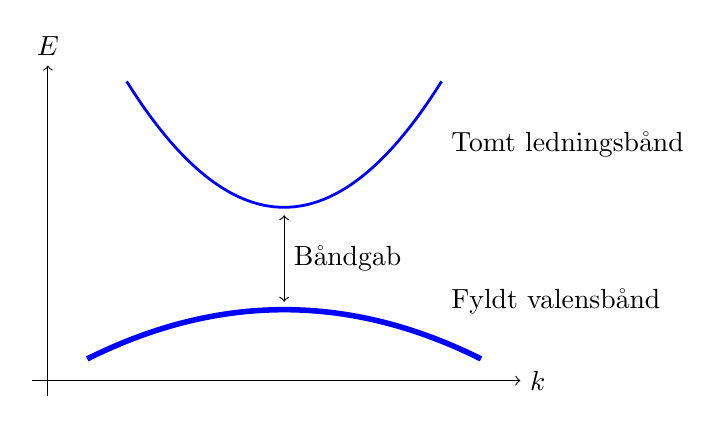
\begin{tikzpicture}
    \draw [->] (-3.2,0) -- (3,0);
    \node [right] at (3,0) {$k$};
    \draw [->] (-3,-.2) -- (-3,4);
    \node [above] at (-3,4) {$E$};

    \draw [color=Blue, line width = 2pt, domain=-2.5:2.5,
    samples=40, smooth]
    plot (\x, {-.1*\x*\x + .9});

    \draw [color=Blue, line width = 1pt, domain=-2:2,
    samples=40, smooth]
    plot (\x, {.4*\x*\x + 2.2});

    \draw [<->] (0,1) -- (0,2.1);
    
    \node [right] at (2,1) {Fyldt valensbånd};
    \node [right] at (2,3) {Tomt ledningsbånd};
    \node [right] at (0,1.55) {Båndgab};
  \end{tikzpicture}  
  \caption{En isolator er karakteriseret ved et båndgab mellem det
    højeste fyldte og nederste ikke-fyldte energibånd.}
  \label{fig:isolator}
\end{figure}


En særlig type af isolatorer kaldes topologiske isolatorer, fordi de
besidder særlige egenskaber, der kan beskrives vha. den matematiske
diciplin topologi. Topologi handler bl.a. om at karakterisere objekter
vha. tal, der er uændrede under glatte deformationer af objektet. I
denne forstand er en kaffekop og en doughnut ens, men forskellig fra
en fodbold -- her er det antallet af huller i objektet, der er det
invariante topologiske tal, der er uændret under glatte
deformationer. I en topologisk isolator kan energibåndene
karakteriseres vha. lignende topologisk invariante tal. Systemets
topologiske egenskaber, såsom eksistensen af kvantemekaniske
tilstande, der lever på kanten af systemet, er umådeligt robuste,
fordi netop deformationer af systemet kun kan ændre det topologisk
invariante tal i ganske særlige tilfælde. Denne robusthed overfor støj
er en af årsagerne til, at topologiske materialer er blevet spået en
fremtid indefor diverse kvanteteknologier. Opdagelsen af topologiske
materialer og stoffers overgang mellem forskellige topologiske faser
gav i år (2016) Thouless, Haldane og Kosterlitz Nobelprisen i fysik.


\section{Chern-isolatoren}

Vi skal nu beskæftige os med en specifik model for en topologisk
isolator, der dog belyser nogle meget centrale og generelle
pointer. Betragt følgende 2-niveau Hamilton-operator:
\begin{equation}
  \label{eq:ci-hamilton}
  H (\v k) = \v h (\v k) \cdot \boldsymbol{\sigma}
  \; ,
  \quad
  \text{hvor}
  \quad
  \v h (\v k) =
  \begin{bmatrix}
    \sin k_x \\ \sin k_y \\ r + \cos k_x + \cos k_y
  \end{bmatrix}
\end{equation}
Her afhænger Hamilton-operatoren af 2D-bølgevektoren $\v k = (k_x,
k_y)$, og $\boldsymbol{\sigma} = (\sigma_x, \sigma_y, \sigma_z)$
er Paulis sigma-matricer. De to energiniveauer er givet ved
\begin{equation}
  \label{eq:ci-energi}
    E_\pm(\v k) = \pm
  \sqrt{\sin^2 k_x + \sin^2 k_y + (r + \cos k_x + \cos k_y)^2} \; .
\end{equation}
Denne model kan bruges til at beskrive en isolator, hvor de to
energiniveuer er hhv. valensbåndet og ledningsbåndet fra
figur~\ref{fig:isolator} (teknisk set er energibåndene nu
2D-overflader).

\begin{itemize}
\item Vis, at Hamilton-operatoren \eqref{eq:ci-hamilton} er hermitisk.
\item Vis, at energiniveauerne er givet ved \eqref{eq:ci-energi}.
\item Argumentér for, at Brillouin-zonen (BZ) er 2D-overfladen givet ved
  $0 \leq k_x, k_y < 2\pi$.
\item Er det muligt at lukke båndgabet i isolatoren? For hvilke
  værdier af $r$ er det muligt, og hvor i BZ sker det?
\item Plot de to energibånd (energioverflader) over BZ for forskellige
  valg af parameteren $r$. Bekræft, at båndgabet lukkes for de værdier
  af $r$, som I fandt ovenfor.
\end{itemize}

Vi kan knytte et topologisk invariant tal, kaldet Chern-tallet, til
hvert energibånd. Chern-tallet er et heltal, der afhænger af værdien
af parameteren $r$. Hvis Chern-tallet ændrer sig, må det derfor
springe i skridt af hele tal, også selvom $r$ ændres
kontinuert. Chern-tallet for grundtilstandsbåndet er givet ved:
\begin{equation}
  \label{eq:cherntal}
  C_- = \frac{1}{4\pi} \int_\text{BZ} d^2 k \;
  \v n \cdot (\partial_{k_x} \v n \times \partial_{k_y} \v n) \; ,
\end{equation}
hvor $\v n = \v h / |\v h|$ er enhedsvektoren, og dermed angiver et
punkt på en sfære med radius 1 (kaldet Bloch-sfæren). Integralet er
over hele BZ, som kan afbildes som en torus (doughnut) med omkreds
$2\pi$ i begge retninger, idet $k_x$ og $k_x + 2\pi$ pr. periodicitet
er fysisk ækvivalente punkter (tilsvarende for $k_y$). Integralet over
hele BZ er altså et dobbeltintegrale over $k_x$ og $k_y$, der begge
integreres fra $0$ til $2\pi$. Chern-tallet for det øverste energibånd
er $C_+ = - C_-$.

\begin{figure}[htbp]
  \centering
  \includegraphics[width=.8\textwidth]{TorustoSpheFigCut}
  \caption{Chern-tallet for det nederste energibånd $C_-$ er det antal
    gange $\v n (\v k)$ overstryger Bloch-sfæren (regnet med fortegn)
    idet der integreres over BZ.}
  \label{fig:mapping}
\end{figure}

\begin{itemize}
\item Argumentér for, at $d^2k \, (\partial_{k_x} \v n
  \times \partial_{k_y} \v n) = \partial_{k_x} \v n \, dk_x \times
  \partial_{k_y} \v n \, dk_y$ er en infinitesimal arealvektor vinkelret
  på Bloch-sfæren.
\item Argumentér for, at $d^2k \; \v n \cdot (\partial_{k_x} \v n
  \times \partial_{k_y} \v n) = \v n \cdot ( \partial_{k_x} \v n
    \, dk_x \times \partial_{k_y} \v n \, dk_y )$ er et
  infinitesimalt areal på Bloch-sfæren (regnet med fortegn).
\item Konkludér nu, at integralet $\int_\text{BZ} d^2k \; \v n \cdot
  (\partial_{k_x} \v n \times \partial_{k_y} \v n)$ er det areal
  (regnet med fortegn), som $\v n (\v k)$ overstryger idet der
  integreres over BZ. Da Bloch-sfærens overfladeareal er $4\pi$, er
  $C_-$ altså den andel af sfæren, som $\v n (\v k)$ overstryger i
  løbet af integrationen over BZ.
\end{itemize}
At $C_-$ endda må være et heltal vil vi vise i det følgende. Vi vil
derfor overveje, hvad der sker, når man integrerer over BZ. Formelt
skrives det som et dobbeltintegrale:
\begin{equation}
  \label{eq:chern-di}
  C_- = \frac{1}{4\pi}
  \int\limits_0^{2\pi} dk_x \int\limits_0^{2\pi} dk_y \;
  \v n \cdot
  (\partial_{k_x} \v n \times \partial_{k_y} \v n) \; .
\end{equation}

\begin{itemize}
\item Hold $k_x$ fast og betragt det inderste (linje-)integrale over
  $k_y$ i ligning~\eqref{eq:chern-di}. Argumentér for, at $\v n(\v k)$
  overstryger en orienteret lukket kurve $\mathcal{P}(k_x)$ på
  Bloch-sfæren idet $k_y$ varieres fra $0$ til $2\pi$.
\item Såfremt $\v n(\v k)$ er veldefineret, vil $\mathcal{P}(k_x)$
  ændres kontinuert som $k_x$ varieres. Argumentér for, at vi starter
  og slutter med den samme kurve idet $k_x$ varieres fra $0$ til
  $2\pi$.
\item Antag, at $\mathcal{P}(k_x)$ ikke ændrer orientering idet $k_x$
  varieres fra $0$ til $2\pi$. Argumentér for, at da vil $C_- = 0$.
\item Hvad skal $\mathcal{P}(k_x)$ opfylde for at få $C_- \neq 0$?
  Hvordan kan dette lade sig gøre geometrisk?
\end{itemize}

Med det specifikke $\v h (\v k)$ givet i
ligning~\eqref{eq:ci-hamilton} kan $C_-$ antage værdierne $0, \pm 1$
afhænging af værdien af $r$. Et Chern-tal på $0$ fås ved at $\v n (\v
k)$ først overstryger et område på Bloch-sfæren, og derefter
overstryger det samme område med modsat fortegn, hvorimod et Chern-tal
på $\pm 1$ fås når $\v n(\v k)$ overstryger hele sfæren én gang. Vi
vil nu undersøge, hvordan $C_-$ afhænger af $r$.

\begin{itemize}
\item Eftersom $C_-$ altid er et heltal, kan værdien af $C_-$ ikke
  ændres ved at ændre $\v n (\v k)$ på kontinuert måde. Kun når $\v n
  (\v k)$ går hen og bliver diskontinuert, kan $C_-$ ændres sig (i
  spring af heltal). For hvilke værdier af $r$ kan det ske, og i
  hvilke punkter i BZ? Hvad sker der rent fysisk i disse tilfælde?
  Argumenter for, at $C_-$ ikke er veldefineret for disse værdier af
  $r$.
\item Angiv de fire intervaller for $r$, hvor $C_-$ kan have
  forskellig værdi.
\item Hvad er $C_-$ når $r < -2$ og $r > 2$?
\end{itemize}

Vi vil i det følgende fokusere på området omkring $r=-2$ og beregne
$C_-$ når $-2 < r < 0$. Analysen vil bygge på en beregning af bidraget
til $C_-$ fra området omkring $\v k = (0,0)$ for $r$ omkring
$-2$. Definér $m = r + 2$, dvs. vi er interesserede i $C_-$ omkring
$m=0$.

\begin{itemize}
\item Vis, at når $\v k \approx (0,0)$, er
  \[
  \v h (\v k) \approx 
  \begin{bmatrix}
    k_x \\ k_y \\ m
  \end{bmatrix}
  \; .
  \]
  Med andre ord er Hamilton-operatoren
  \begin{equation}
    \label{eq:ci-dirac}
    H(\v k ) \approx k_x \sigma_x + k_y \sigma_y + m \sigma_z \; .
  \end{equation}
\item Vis, at når $\v k \approx (0,0)$ er
  \begin{equation}
    \label{eq:ci-lin-int}
    \v n \cdot (\partial_{k_x} \v n \times \partial_{k_y} \v n)
    \approx \frac{m}{(k^2 + m^2)^{3/2}} \; ,
  \end{equation}
  hvor $k^2 = k_x^2 + k_y^2$.
\item Beregn hvor meget området omkring $\v k = (0,0)$ bidrager til
  Chern-tallet $C_-$. Dette gøres ved at indsætte
  udtrykket~\eqref{eq:ci-lin-int} i \eqref{eq:cherntal}, men i stedet
  for at integrere over hele BZ, skal I kun integrere i omegnen af $\v
  k = (0,0)$. Dette kan fx gøres ved at integrere over en cirkelskive
  med centrum i $\v k = (0,0)$ og radius $R$, og dernæst lade $R
  \rightarrow 0$. Vis, at bidraget til $C_-$ er $-1/2$ når $m
  \rightarrow 0^-$, og $1/2$ når $m \rightarrow 0^+$. (Pas på med
  rækkefølgen, I tager grænseværdierne for $m$ og $R$ i -- de
  kommuterer nemlig ikke!)
\item Argumentér for, at den del af BZ, som I ikke integrerede over,
  bidrager med $1/2$ til $C_-$ når $m \rightarrow 0^-$. Da integranden
  i \eqref{eq:cherntal} er veldefineret i denne del af BZ også når
  $m=0$, giver denne del ligeledes bidraget $1/2$ når $m \rightarrow
  0^+$. Hvad er $C_-$ når $-2 < r < 0$?
\end{itemize}

I har nu beregnet $C_-$ når $r < 0$. Vha. lignende argumenter kan man
beregne $C_-$ når $r > 0$, om man finder, at Chern-tallet er en ulige
funktion af $r$, dvs. at $C_- (r) = - C_- (-r)$.

\begin{itemize}
\item Plot Chern-tallet for hvert energibånd, $C_\pm(r)$, som
  funktion af $r$.
\end{itemize}

Ved at variere parameteren $r$ kan man altså ændre Chern-tallene på
energiniveauerne. Når dette sker taler man om en topologisk
faseovergang.

%Som I har set er en topologisk faseovergang forbundet
%med, at energien bliver nul og altså eksistensen af kvantemekaniske
%tilstande med nul energi (som på en måde er gratis tilstande set fra
%et energetisk perspektiv).

\section{Generelt 2-niveau-system}

Hvis I har tid, kan I prøve at se på et generelt 2-niveau-system med
en $\v k$-afhængig Hamilton-operator, hvor Chern-isolatoren altså er
et specialtilfælde. En generel Hamilton-operator kan skrives som
\begin{equation}
  \label{eq:generel-hamilton}
  H (\v k) = \v h (\v k) \cdot \boldsymbol{\sigma} \; ,
\end{equation}
hvor $\v h (\v k)$ er en general 3D-vektor med $\v k$-afhængige
indgange.

\begin{itemize}
\item Vis, at denne Hamilton-operator beskriver alle
  2-niveau-systemer.
\item Hvad er energiniveauerne?
\item Chern-tallet er givet som i forrige afsnit. Gennemgå
  argumenterne for, at Chern-tallet er et heltal og overbevis jer om,
  at dette også gælder for et generelt 2-niveau-system.
\item Vis, at Chern-tallet kun kan ændres når båndgabet lukkes
  (dvs. når energiniveauerne bliver udartede).
\end{itemize}





\begin{thebibliography}{9}
  \bibitem{gp}
    G. Grosso \& G. P.  Parravicini: {\it Solid State Physics}, 2nd ed.,
    Academic Press (2014)
  \bibitem{gb} G. M. Bruun: {\it Lecture Notes for Solid State Physics
      II} (2016)
\end{thebibliography}


\end{document}


%%% Local Variables: 
%%% mode: latex
%%% TeX-master: t
%%% End: 
